\section{One dimension}\label{ht:sec:d1}

\subsection{Campaigns}\label{ht:sec:d1-campaigns}
All $d=1$ runs used the solver \code{HT/code/lri\_dressed\_phi4\_hpc} on the symmetry cluster (Perimeter
Institute). There were two campaigns.

\paragraph{\code{dens\_v1} (production, code 33998bb, 2026-10-07 to 10-09).}
\begin{itemize}
\item \emph{Setup.} Consistent window, density basis with $n_z=\HTq{S5}$ (one stored basis per $\Ds$, trained at
 $N_t=24$), auxiliary oscillator basis of $N_{\rm osc}=384$ states.
\item \emph{Grid.} The 13 values $\Ds=0.249$, 0.24, 0.225, 0.2, 0.175, 0.15, 0.125, 0.1, 0.075, 0.05, 0.025, 0.01 and 0.001,
 that is $\eps=1-4\Ds$ from 0.004 to 0.996, at every even $N$ from $\HTq{S1}$ to $\HTq{S2}$: 195 points.
\item \emph{Controls.} Six controls with 24 kept states at $N=36$, 40. Two further controls, at $N=40$ and
 $\Ds=0.025$, $0.01$, stopped at their walltime and are not used.
\item \emph{Execution.} Items were packed on whole nodes (64-core AMD amdq; 40-core Intel preq), with 1 to 16
 threads per item. Items resumed from Newton checkpoints after a cluster-wide node failure and after walltime stops.
\item \emph{Cost.} The longest items took 15\,h ($N=40$, $\Ds=0.025$, 16 threads). The total was about $10^4$
 core-hours of exclusive nodes. Every record carries its configuration, couplings, levels, window table, residuals
 and timing, and a sha256 over its content.
\end{itemize}

\paragraph{\code{prod1--7} (code 4dfd833, 2026-10-02 to 10-05).}
\begin{itemize}
\item \emph{Content.} Energy zero-mode basis with $n_z=24$ to 56, in the raw, consistent and literal prescriptions,
 at $N=12$ to 40: 680 records, about $1.06\times10^4$ core-hours.
\item \emph{Why it was superseded.} At $\Ds\le0.05$ its series needed an $n_z$ that grows with $N$, and their
 extrapolations mixed values of different $n_z$. The production values now come from \code{dens\_v1}.
\item \emph{What is still used.} Its records serve three roles: the inputs of the descendant-identity diagnostic
 (Section~\ref{ht:sec:d1-ident}), the references of the basis check at $N=32$, and the references of the blind-solver
 comparison.
\end{itemize}

\subsection{Extrapolation}\label{ht:sec:d1-extrap}
\paragraph{Fits.} For each $\Ds$ we fit
\begin{equation}
 \DE(N)=\Delta_\infty+aN^{-\omega}\quad\big[{}+bN^{-\omega-1}\ \text{(F2) or }{}+bN^{-2\omega}\ \text{(F3)}\big],\qquad N\ge N_{\min},
 \label{ht:eq:fitN}
\end{equation}
with F1 the two-term form. The fit set is:
\begin{itemize}
\item $N_{\min}=\HTq{S3}$ in steps of 2, giving $\HTq{S4}$ fits per $\Ds$;
\item each fit is a nonlinear least-squares fit from five starting exponents, keeping the best.
\end{itemize}

\paragraph{Acceptance.} A fit is accepted if all three conditions hold:
\begin{itemize}
\item rms residual $<3\times10^{-6}$;
\item $0.2<\omega<4$;
\item $|\Delta_\infty-\DE(N_{\max})|<0.05$.
\end{itemize}
We quote the median of the accepted $\Delta_\infty$ and their half-spread, half the difference between the largest
and the smallest accepted $\Delta_\infty$. It is a model spread, not a standard deviation.

\paragraph{Stability.} A result is \emph{stable} if all three conditions hold:
\begin{itemize}
\item at least five fits are accepted;
\item the median of their fitted $\omega$ is at least 0.45 (a condition on the fits, not on $\omega_{\rm eff}$
 below);
\item the half-spread is at most $2\times10^{-3}$.
\end{itemize}
The median exponents of the stable results lie at $\HTq{S11}$.

\paragraph{Status words.} A stable result is \emph{final} if the local exponent $\omega_{\rm eff}$ below levels off
over the largest cutoffs, and \emph{one-sided} if it still rises, which suggests that the fits overestimate the limit;
this classification is a judgement. A series that turns over and keeps falling has \emph{no limit}. Any other result
that is not stable is \emph{unstable}: we give the range of the accepted fits but no limit. In $d=2,3$,
\emph{finite-$N$} marks values of the truncated model at a given cutoff, with no extrapolation.

\paragraph{Local exponent.} A fit-free check is
\begin{equation}
 \omega_{\rm eff}(N)=-\frac{d\ln\big(d\DE/d\ln N\big)}{d\ln N},
 \label{ht:eq:omegaeff}
\end{equation}
which is constant for a single power law. We evaluate it by finite differences. The slope on a pair of successive
cutoffs, $s=[\DE(N'+2)-\DE(N')]/\ln\frac{N'+2}{N'}$, sits at $\bar N=\sqrt{N'(N'+2)}$. From the slopes on
$[N',N'+2]$ and $[N'+4,N'+6]$ we take $\omega_{\rm eff}=-\ln(s_2/s_1)/\ln(\bar N_2/\bar N_1)$ and label it by
the centre $N=N'+3$ of the four cutoffs, $N=15,19,\dots,35$.

\paragraph{Held-out test.} Fits restricted to $N\le N_{\rm cut}$ predict the cutoffs above $N_{\rm cut}$
(Table~\ref{ht:tab:d1-holdout}).

\subsection{Results}\label{ht:sec:d1-results}
Table~\ref{ht:tab:d1} gives $\DE$ at the largest cutoff and extrapolated. Figure~\ref{ht:fig:d1} shows the strong-coupling
series and their local exponents.

\begin{table}[t]
\centering\small\renewcommand{\arraystretch}{1.15}
\begin{tabular}{@{}l l l l l l@{}}
\toprule
$\Ds$ & $\eps$ & $\DE(N=40)$ & $\DE(N\to\infty)$ & status & NRG\\
\midrule
\inputrows{parts/ht/sections/tab_d1_main.tex}
\bottomrule
\end{tabular}
\caption{$\DE$ in $d=1$ from finite-coupling HT, at the largest cutoff and extrapolated with
Eq.~\eqref{ht:eq:fitN}. Errors in parentheses are half-spreads of the accepted fits (model spreads, not standard
deviations), printed with the paper's rounding rule.
\emph{Weak coupling.} At $\Ds\geq0.15$ these spreads, at most $\HTq{D13}$, are probably optimistic; we judge the
total error there to be about $\HTq{D12}$. At $\Ds=0.249$ this is conservative: the $\eps$ expansion agrees to
$\HTq{P1}$ (Section~\ref{ht:sec:d1-pert}).
\emph{$\Ds=0.075$.} The second error is one-sided: a further rise of $\omega_{\rm eff}$ by 0.2 would lower the limit
by about $\HTq{E6}$.
\emph{$\Ds=0.05$.} The accepted F1 and F2 fits give the range shown, an upper estimate if $\omega_{\rm eff}$ keeps
rising. The F3 fits admit a later turnover and reach the lowest value shown. The data up to $N=40$ cannot decide, so
we quote no limit there, only this range, and none at $\Ds\le0.025$.
The errors do not include the dependence on the window prescription (Section~\ref{ht:sec:d1-model}).
\emph{NRG.} Bosonic NRG of the sub-ohmic spin-boson model~\cite{ht:Bulla:2003rns,ht:Bulla:2005bnrg} (NRG folder, final
table), shown for comparison. Its error is the sum of three convergence diagnostics (chain depth, kept states,
discretization), not a standard deviation; $^{\rm nc}$: not converged in chain depth near $\Ds=\frac14$.}
\label{ht:tab:d1}
\end{table}

\begin{figure}[t]
\centering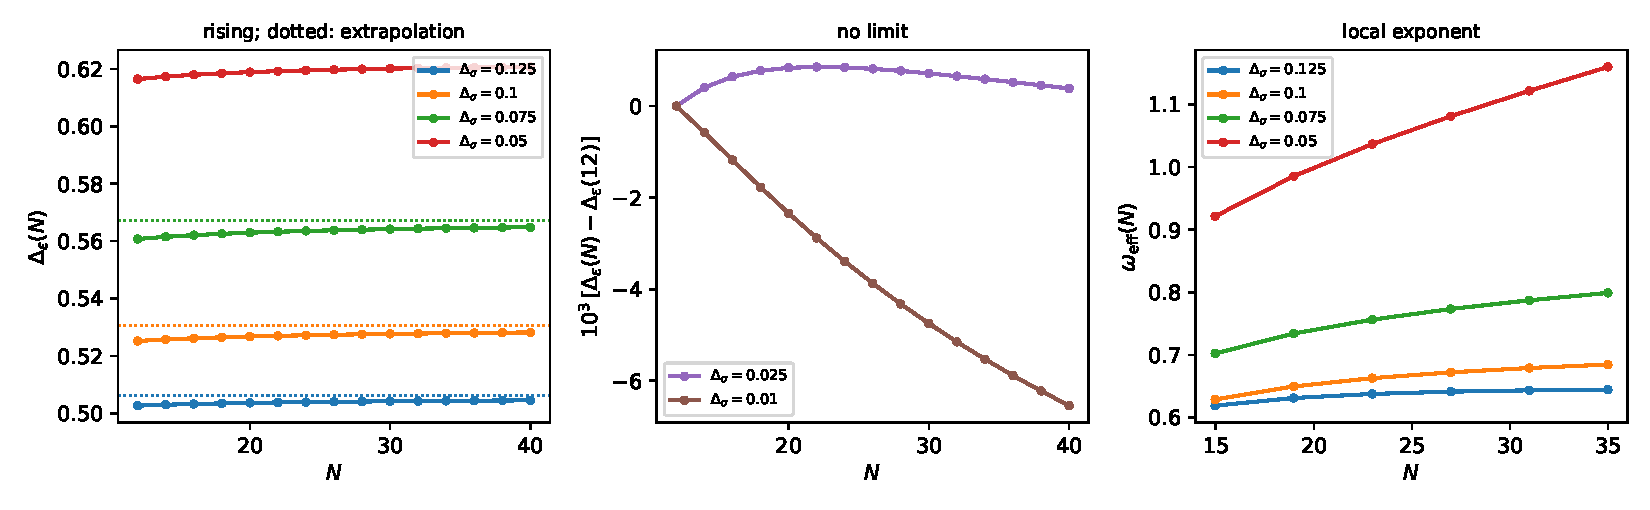
\includegraphics[width=\textwidth]{parts/ht/figures/fig_d1_cutoff.pdf}
\caption{$d=1$, \code{dens\_v1}.
\emph{Left:} $\DE(N)$ at $0.05\le\Ds\le0.125$; the dotted lines are the extrapolations of the stable series
(0.075 to 0.125).
\emph{Middle:} change $\DE(N)-\DE(12)$ at $\Ds=0.025$, which peaks near $N=\HTq{E8}$ and then falls, and at 0.01,
which falls at a nearly constant rate per unit of $\ln N$.
\emph{Right:} the local exponent~\eqref{ht:eq:omegaeff}, which levels off at 0.125 and 0.1 but rises at 0.075 and 0.05.}
\label{ht:fig:d1}
\end{figure}

\paragraph{Weak coupling and the $\eps$ expansion.}\label{ht:sec:d1-pert}
\begin{itemize}
\item At $\Ds=0.249$ the extrapolation differs from the $\eps$ series through $\eps^7$ (GFF folder:
 $C_2=(\pi+4\ln2)/9$, $C_3$ to $C_7$) by $\HTq{P1}$. That is below the $\HTq{P4}$ at which we trust the check,
 because of the series and fit systematics.
\item At $\Ds=0.24$ the value lies within the band $\HTq{P2}$ of the partial sums through $\eps^4$ to $\eps^7$.
\item The blind solver of Section~\ref{ht:sec:checks} computes the weak-coupling coefficient of the truncated model.
 With $\DE=\frac12-\frac\eps6+C_2(N)\eps^2+\dots$, it reproduces
 \begin{equation}
 C_2(N)=\frac{34}{81}+\sum_{n\ \text{even},\,2\le n\le N}v_n\Big[\frac{2}{81(n-\frac12)}+\frac{2}{9n}+\frac{2}{9(n+\frac12)}+\frac{2}{81(n+1)}\Big],\qquad v_n=\frac{(\frac12)_n}{n!},
 \label{ht:eq:C2N}
 \end{equation}
 to at most $3\times10^{-7}$ for $N=0$ to 16, raw and corrected. The limit of $C_2(N)$ is the GFF value; the
 approach is like $N^{-1/2}$.
\end{itemize}

\paragraph{Intermediate coupling.}
\begin{itemize}
\item The extrapolations are final for $\Ds\geq0.1$.
\item At $0.075\le\Ds\le0.125$ they add $\HTq{E7}$ to the $N=40$ values.
\item Over $15\le N\le35$ the local exponent levels off:
 \begin{itemize}
 \item at $\HTq{E1}$ for $\Ds=0.125$;
 \item at $\HTq{E2}$ for 0.1.
 \end{itemize}
\item It rises instead, over the same range of $N$:
 \begin{itemize}
 \item $\HTq{E3}$ at 0.075;
 \item $\HTq{E4}$ at 0.05.
 \end{itemize}
\item A rising $\omega_{\rm eff}$ precedes the turnover seen at $\Ds=0.025$ and suggests that the fits overestimate
 the limit. This is why 0.075 carries a one-sided error. The classification final versus one-sided is a judgement
 based on these trends; they differ only modestly between 0.1 and 0.075.
\item At weak coupling $\omega_{\rm eff}$ also rises slowly ($\HTq{E11}$ at $\Ds=0.249$), but the bias it implies is
 below $\HTq{E12}$.
\item Fits restricted to $N\le32$ predict $N=34$--40 to $\HTq{E5}$ (Table~\ref{ht:tab:d1-holdout}).
\end{itemize}

\begin{table}[t]
\centering\footnotesize\renewcommand{\arraystretch}{1.1}
\begin{tabular}{@{}l c c c c c c@{}}
\toprule
$\Ds$ & $\omega_{\rm eff}(15)$ & (19) & (23) & (27) & (31) & (35)\\
\midrule
\inputrows{parts/ht/sections/tab_d1_omegaeff.tex}
\bottomrule
\end{tabular}
\caption{Local exponent~\eqref{ht:eq:omegaeff} of the $d=1$ series, labelled by the centre of its four cutoffs.
Held-out test: fits on $N\le32$ predict the values at $N=34$--40 to within $\HTq{E5}$ at every $\Ds\ge0.05$, inside
the spread of the predictions. The test passes also at $\Ds=0.025$, where the series has no limit, so it checks the
fits only within the range of the data, not their limit. All values:
\code{results/HT\_1d/holdout\_and\_local\_exponent.md}.}
\label{ht:tab:d1-holdout}
\end{table}

\paragraph{Strong coupling.}
\begin{itemize}
\item \emph{$\Ds=0.05$.} The series still rises at $N=40$. The accepted F1 and F2 fits give $\HTq{D10}$, a range
 that contains the NRG value of Table~\ref{ht:tab:d1}. The F3 fits reach down to $\HTq{D11}$. Their low branch moves up as cutoffs are
 added, which mildly argues against a turnover.
 The rising $\omega_{\rm eff}$ argues the other way. No value is quoted.
\item \emph{$\Ds\le0.025$.} The corrected sequence does not converge.
 \begin{itemize}
 \item At 0.025 it peaks near $N=\HTq{E8}$ and then falls ever faster, reaching $\HTq{E9}$ per unit of $\ln N$ at
 $N=40$.
 \item At 0.01 it falls at a constant $\HTq{E10}$ per unit of $\ln N$.
 \item At 0.001 it falls slowly but lies $\HTq{C3}$ above the NRG value.
 \end{itemize}
 The zero-mode basis is converged and the solver is verified, so this is a property of the window model, not of the
 numerics. The uncorrected truncation converges, but to values that violate Eq.~\eqref{ht:eq:v}
 (Table~\ref{ht:tab:d1-ident}).
\end{itemize}

\subsection{Model dependence and the comparison with NRG}\label{ht:sec:d1-model}
The errors of Table~\ref{ht:tab:d1} are half-spreads of one family of fits (F1--F3) on one prescription. They do not cover two
further model dependences, which we measure on the shipped records
(\code{public/model\_dependence\_ht1d.py}, table in \code{results/HT\_1d/model\_dependence.md}).
\begin{itemize}
\item \emph{Tail model.} We tried two alternative descriptions of the approach $N\to\infty$ of the same window series:
 \begin{itemize}
 \item F4, Eq.~\eqref{ht:eq:fitN} with two free exponents;
 \item a local exponent continued linearly in $\ln N$ from its last four values, with the slope at $N=40$ integrated
 to infinity.
 \end{itemize}
 Both move the limit down by at most $\HTq{M3}$ at $0.075\le\Ds\le0.125$, of the order of the fit half-spread.
\item \emph{Prescription.} The same truncation without the window (raw, energy zero-mode basis) extrapolates, with
 the same fits, to limits $\HTq{M6}$ below the window limits at $\Ds=0.125$, 0.1 and 0.075, respectively.
 \begin{itemize}
 \item Neither prescription satisfies the descendant identities in the limit (Table~\ref{ht:tab:d1-ident}), so the
 limit of the truncated model depends on the prescription at this level.
 \item At $\Ds\ge0.15$ the two prescriptions agree to $\HTq{M7}$ or better.
 \end{itemize}
\end{itemize}
The prescription dependence, $\HTq{M10}$ at $0.075\le\Ds\le0.125$, is thus as large as the gap to NRG below. We do
not combine these shifts into an error. The truncation has no strict error bar, and an error built after the gap to
NRG had been seen would make the comparison read as agreement within errors. The errors of Table~\ref{ht:tab:d1} stay
the fit spreads. The window limit is expected to be the better of the two, since its $\sigma$ descendant violation is
$\HTq{V2}$ times smaller.

\paragraph{Comparison with NRG.} We compare with the final NRG values of Table~\ref{ht:tab:d1} (NRG folder). Their
errors are sums of three convergence diagnostics, not standard deviations.
\begin{itemize}
\item HT lies above NRG at all six points $0.075\le\Ds\le0.2$, by up to $\HTq{C1}$.
\item The differences are $\HTq{C5}$ to $\HTq{C1}$ at $0.075\le\Ds\le0.15$, and below $\HTq{C6}$ at 0.175 and 0.2.
\item At $\Ds=0.125$, 0.1 and 0.075 the differences are $\HTq{C2}$. They are at least five times both the fit
 half-spreads of Table~\ref{ht:tab:d1} and the NRG errors, and of the size of the prescription dependence.
\item NRG lies between the raw and the window limits at these three points.
\item NRG also lies inside the fit-free bracket $[\DE(40),\,\DE(40)+\frac{d\DE/d\ln N}{\omega_{\rm eff}}]$ of the
 window series at every $0.075\le\Ds\le0.2$. That bracket holds if $\DE(N)$ keeps rising and $\omega_{\rm eff}$
 does not decrease beyond $N=40$.
\end{itemize}
We do not assume that either method is right. The Monte Carlo values that the MC folder labels \emph{accepted}
(MC column of the $d=1$ results table of Ref.~\cite{ht:paper}) also lie above NRG at these three couplings, on the same side as HT, but their
systematic errors exceed the HT--NRG differences, so they cannot decide between the two. The resummed expansions cannot decide at this coupling
(\code{Resummation/} folder). The HT values at
$0.075\le\Ds\le0.125$ are limits of the window-corrected truncation at their fit errors. As estimates of the CFT
they depend on the truncation prescription by the shifts above, which are as large as the gap to NRG.

\subsection{Descendant identities}\label{ht:sec:d1-ident}
Table~\ref{ht:tab:d1-ident} gives the level-1 violations, Eq.~\eqref{ht:eq:v}, at $N=28$, raw and with the window, from
the identity diagnostic run on the \code{prod1--7} records. The other cutoffs are in
\code{results/HT\_1d/identity\_violations.md}.
\begin{itemize}
\item The raw violations do not decay with $N$ over $N=16$--28 and grow with the coupling. At $\Ds\le0.1$ they range
 over $\HTq{V1}$.
\item The window reduces the $\sigma$ violation by $\HTq{V2}$ times at $\Ds\le0.15$.
\item At $\eps\ge0.6$ non-decaying residuals of about $\HTq{V3}$ remain for $\sigma$ and $\phi^3$, and up to
 $\HTq{V4}$ for $\varepsilon$ at $\Ds\le0.05$.
\end{itemize}

\begin{table}[t]
\centering\footnotesize\renewcommand{\arraystretch}{1.1}
\begin{tabular}{@{}l r r r r r r@{}}
\toprule
 & \multicolumn{3}{c}{raw} & \multicolumn{3}{c}{window}\\
\cmidrule(lr){2-4}\cmidrule(l){5-7}
$\Ds$ & $\sigma$ & $\phi^3$ & $\varepsilon$ & $\sigma$ & $\phi^3$ & $\varepsilon$\\
\midrule
\inputrows{parts/ht/sections/tab_d1_ident.tex}
\bottomrule
\end{tabular}
\caption{Level-1 descendant violations $v_1$ at $N=28$, raw and with the consistent window, in the energy zero-mode
basis of \code{prod1--7}: $n_z=24$ at $\Ds\ge0.1$, 32 below. The $\varepsilon$ columns use the first excited
even state. $^a$:~ambiguous identification with the free $L_{-1}$. In the CFT all entries vanish.}
\label{ht:tab:d1-ident}
\end{table}
